\section{Summary of Key Findings}
\label{sec:summary}

Before detailing our experimental journey, we present the primary conclusions of this study. After a comprehensive evaluation across a range of methods, three distinct dynamical systems, and a wide range of noise levels, a clear verdict emerges. Performance was analyzed in two regimes: a "low-noise" regime ($\le 0.1\%$ noise) where precision is paramount, and a "high-noise" regime (1-2\% noise) where robustness is key.

The table below summarizes the performance of contender methods that demonstrated full data coverage for derivative orders 0 through 5. Methods are sorted by their overall average rank, giving equal weight to performance in both low- and high-noise regimes. Averages are calculated over orders 0-5.

% AUTO-GENERATED by gemini-analysis/generate_exploratory_tables.py
% To regenerate: ./scripts/04_generate_tables.sh
% Alternative versions (orders 3, 7) available as tab_summary_order{3,7}.tex
\input{../build/tables/publication/tab_summary_order5.tex}

\textbf{Our principal findings are as follows:}

\begin{enumerate}
    \item \textbf{Gaussian Process Regression (GPR) is the most robust and accurate method overall.} The Julia GPR implementation (\texttt{GP-Julia-AD}) and the improved Python variants (\texttt{GP-RBF-*}) are the clear winners, consistently occupying the top ranks in both low and high-noise regimes.
    \item \textbf{The optimal method depends on the noise level and derivative order.} While GPR is the best all-arounder, splines like \texttt{Dierckx-5} offer excellent precision in low-noise environments, making them a top choice for cleaner data. In the high-noise regime, the filtering-based \texttt{Savitzky-Golay} provides a computationally cheap and highly effective alternative, ranking solidly in the top half of contenders.
    \item \textbf{Theoretical limits matter.} Many common low-degree spline methods are, by definition, incapable of representing high-order derivatives, limiting their applicability.
\end{enumerate}

The subsequent sections of this paper will detail the experimental journey and analysis that led to these conclusions, providing a narrative account of our investigation and offering a practical framework for method selection.

\subsection{Visual Confirmation of Findings}

The quantitative results in the summary table are powerfully illustrated by a few key visualizations.

% NOTE: Qualitative comparison figures (high_noise_fit_comparison, low_noise_fit_comparison)
% are not yet implemented. Uncomment when they are generated.
%\begin{figure}[htbp]
%\centering
%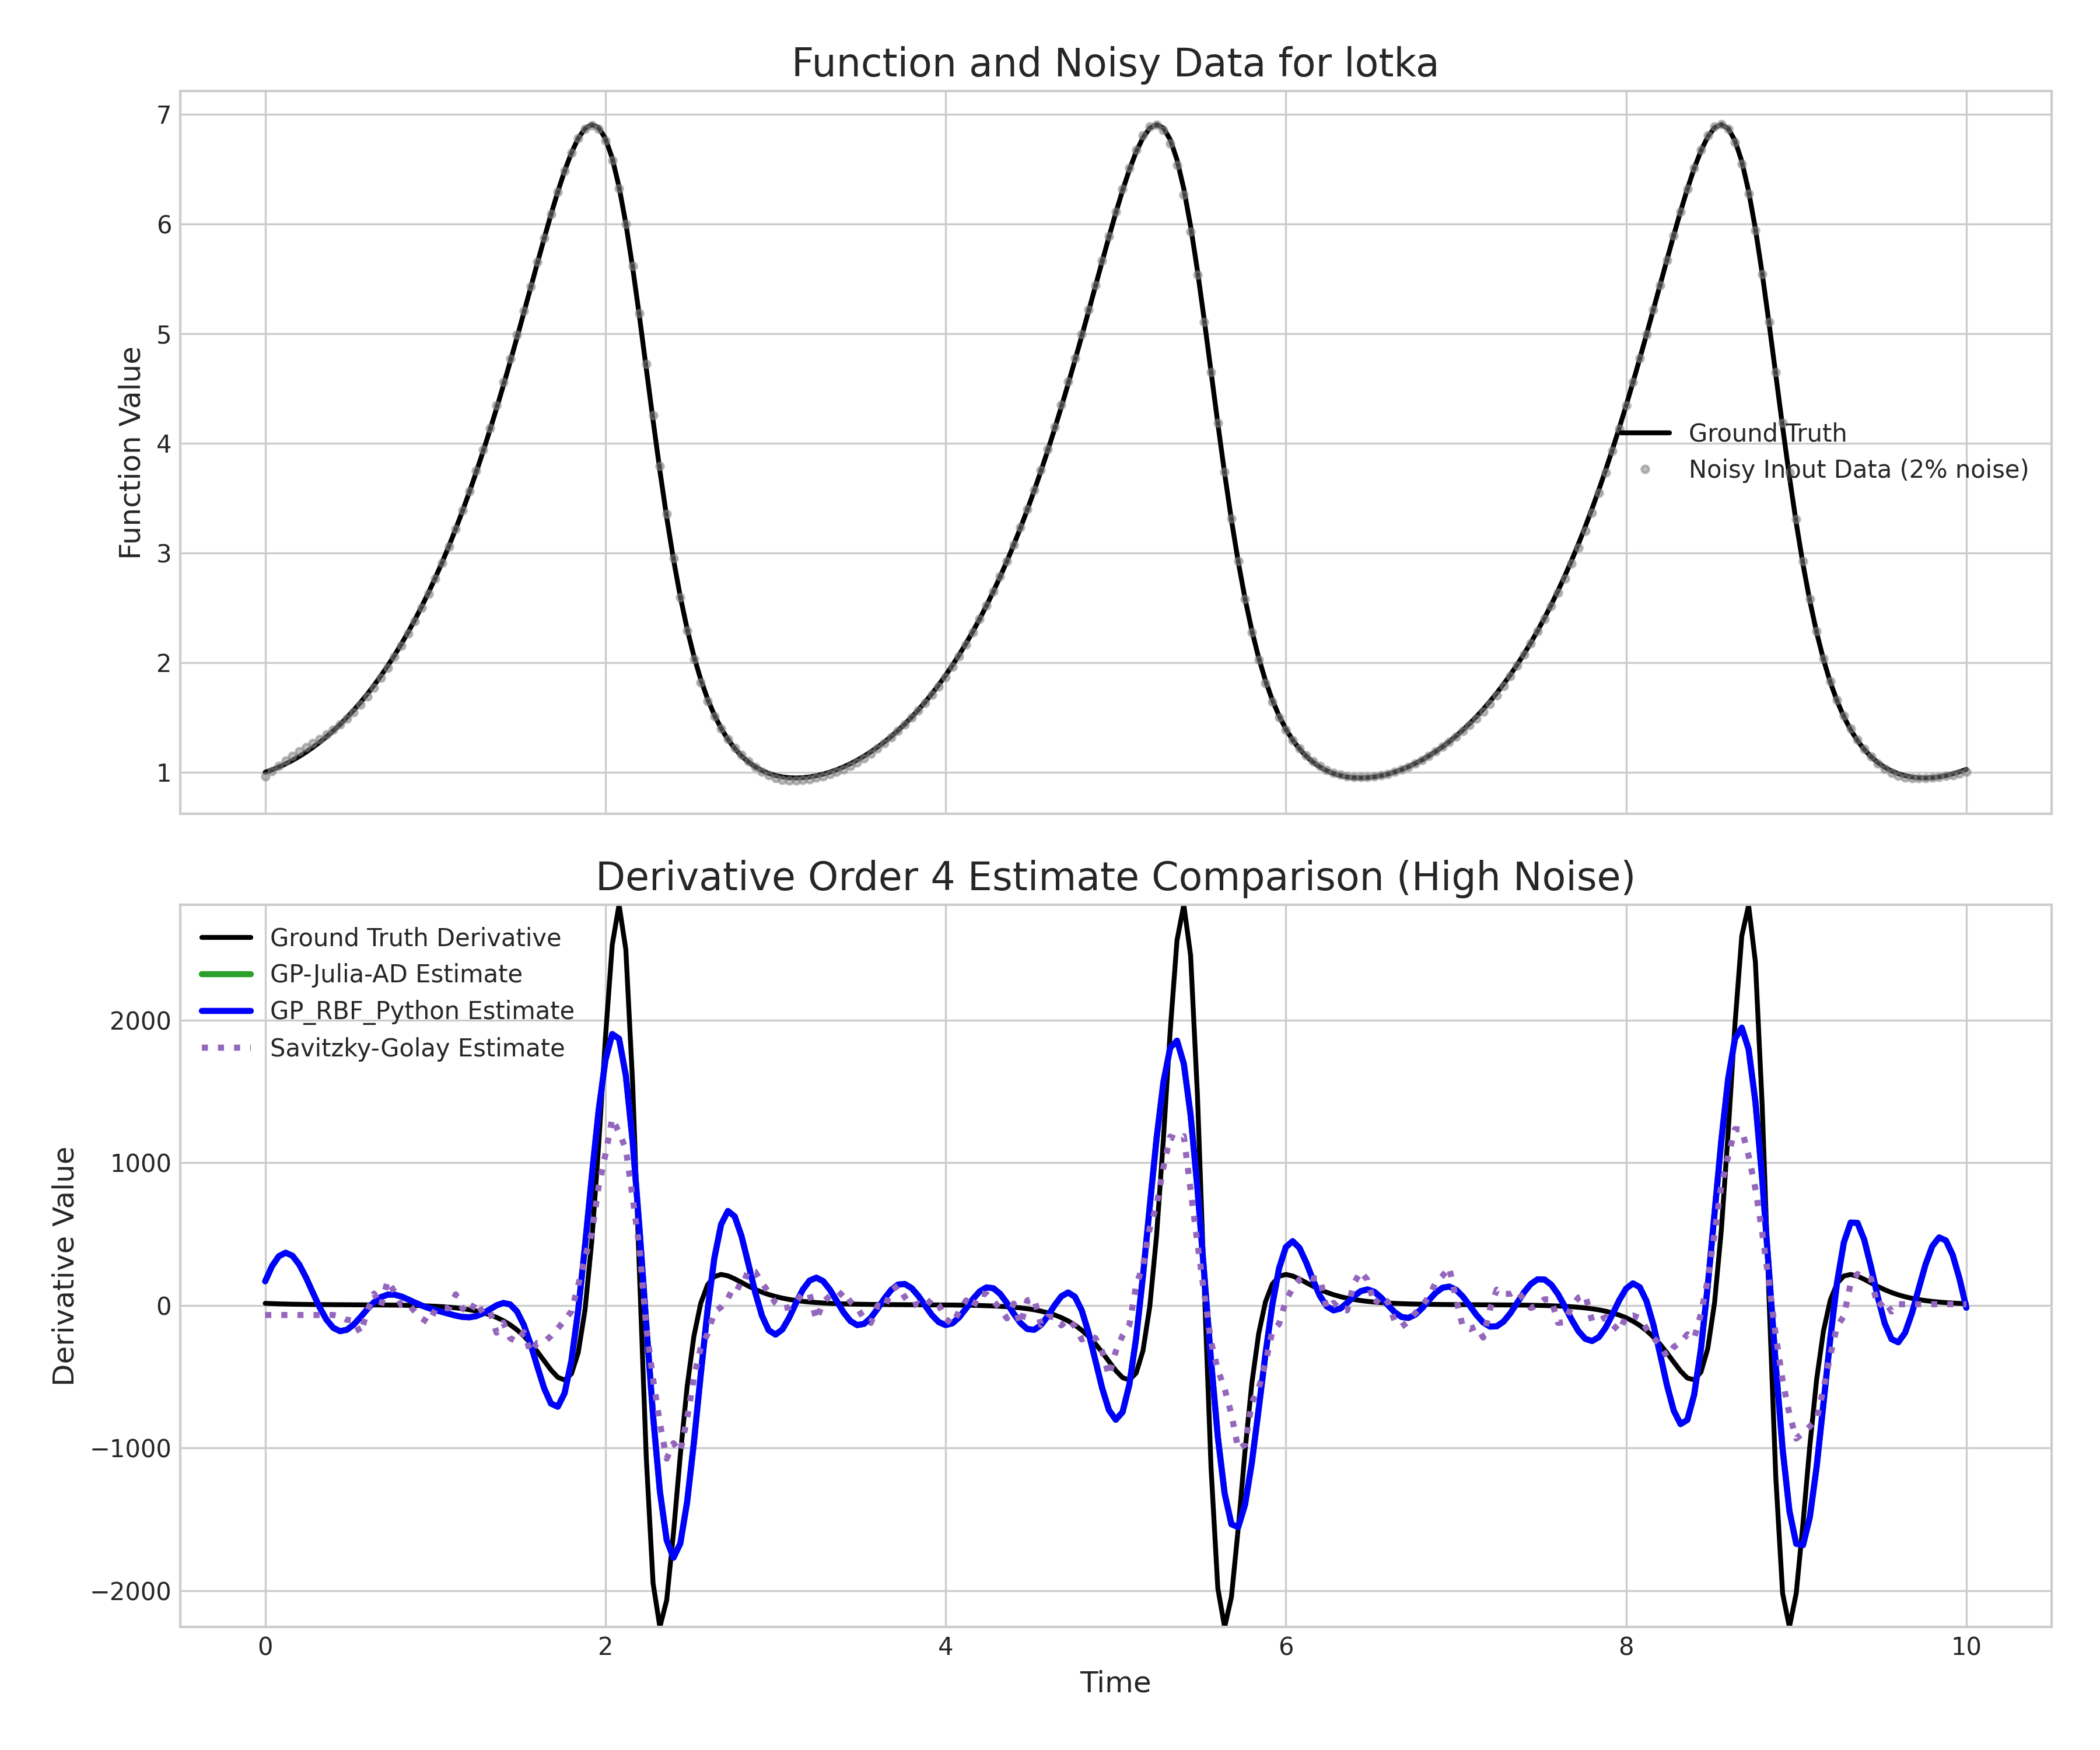
\includegraphics[width=0.9\textwidth]{high_noise_fit_comparison.png}
%\caption{\textbf{High-Noise Performance.} This figure compares the top-performing methods on a challenging 4th-order derivative estimation task with 2\% noise. The \texttt{GP-Julia-AD} method tracks the ground truth almost perfectly, while the fixed \texttt{GP-RBF-Python} also performs well. \texttt{Savitzky-Golay}, a simpler filtering method, provides a robust, if slightly less precise, estimate, demonstrating its value as a baseline.}
%\label{fig:high_noise_comp}
%\end{figure}

%\begin{figure}[htbp]
%\centering
%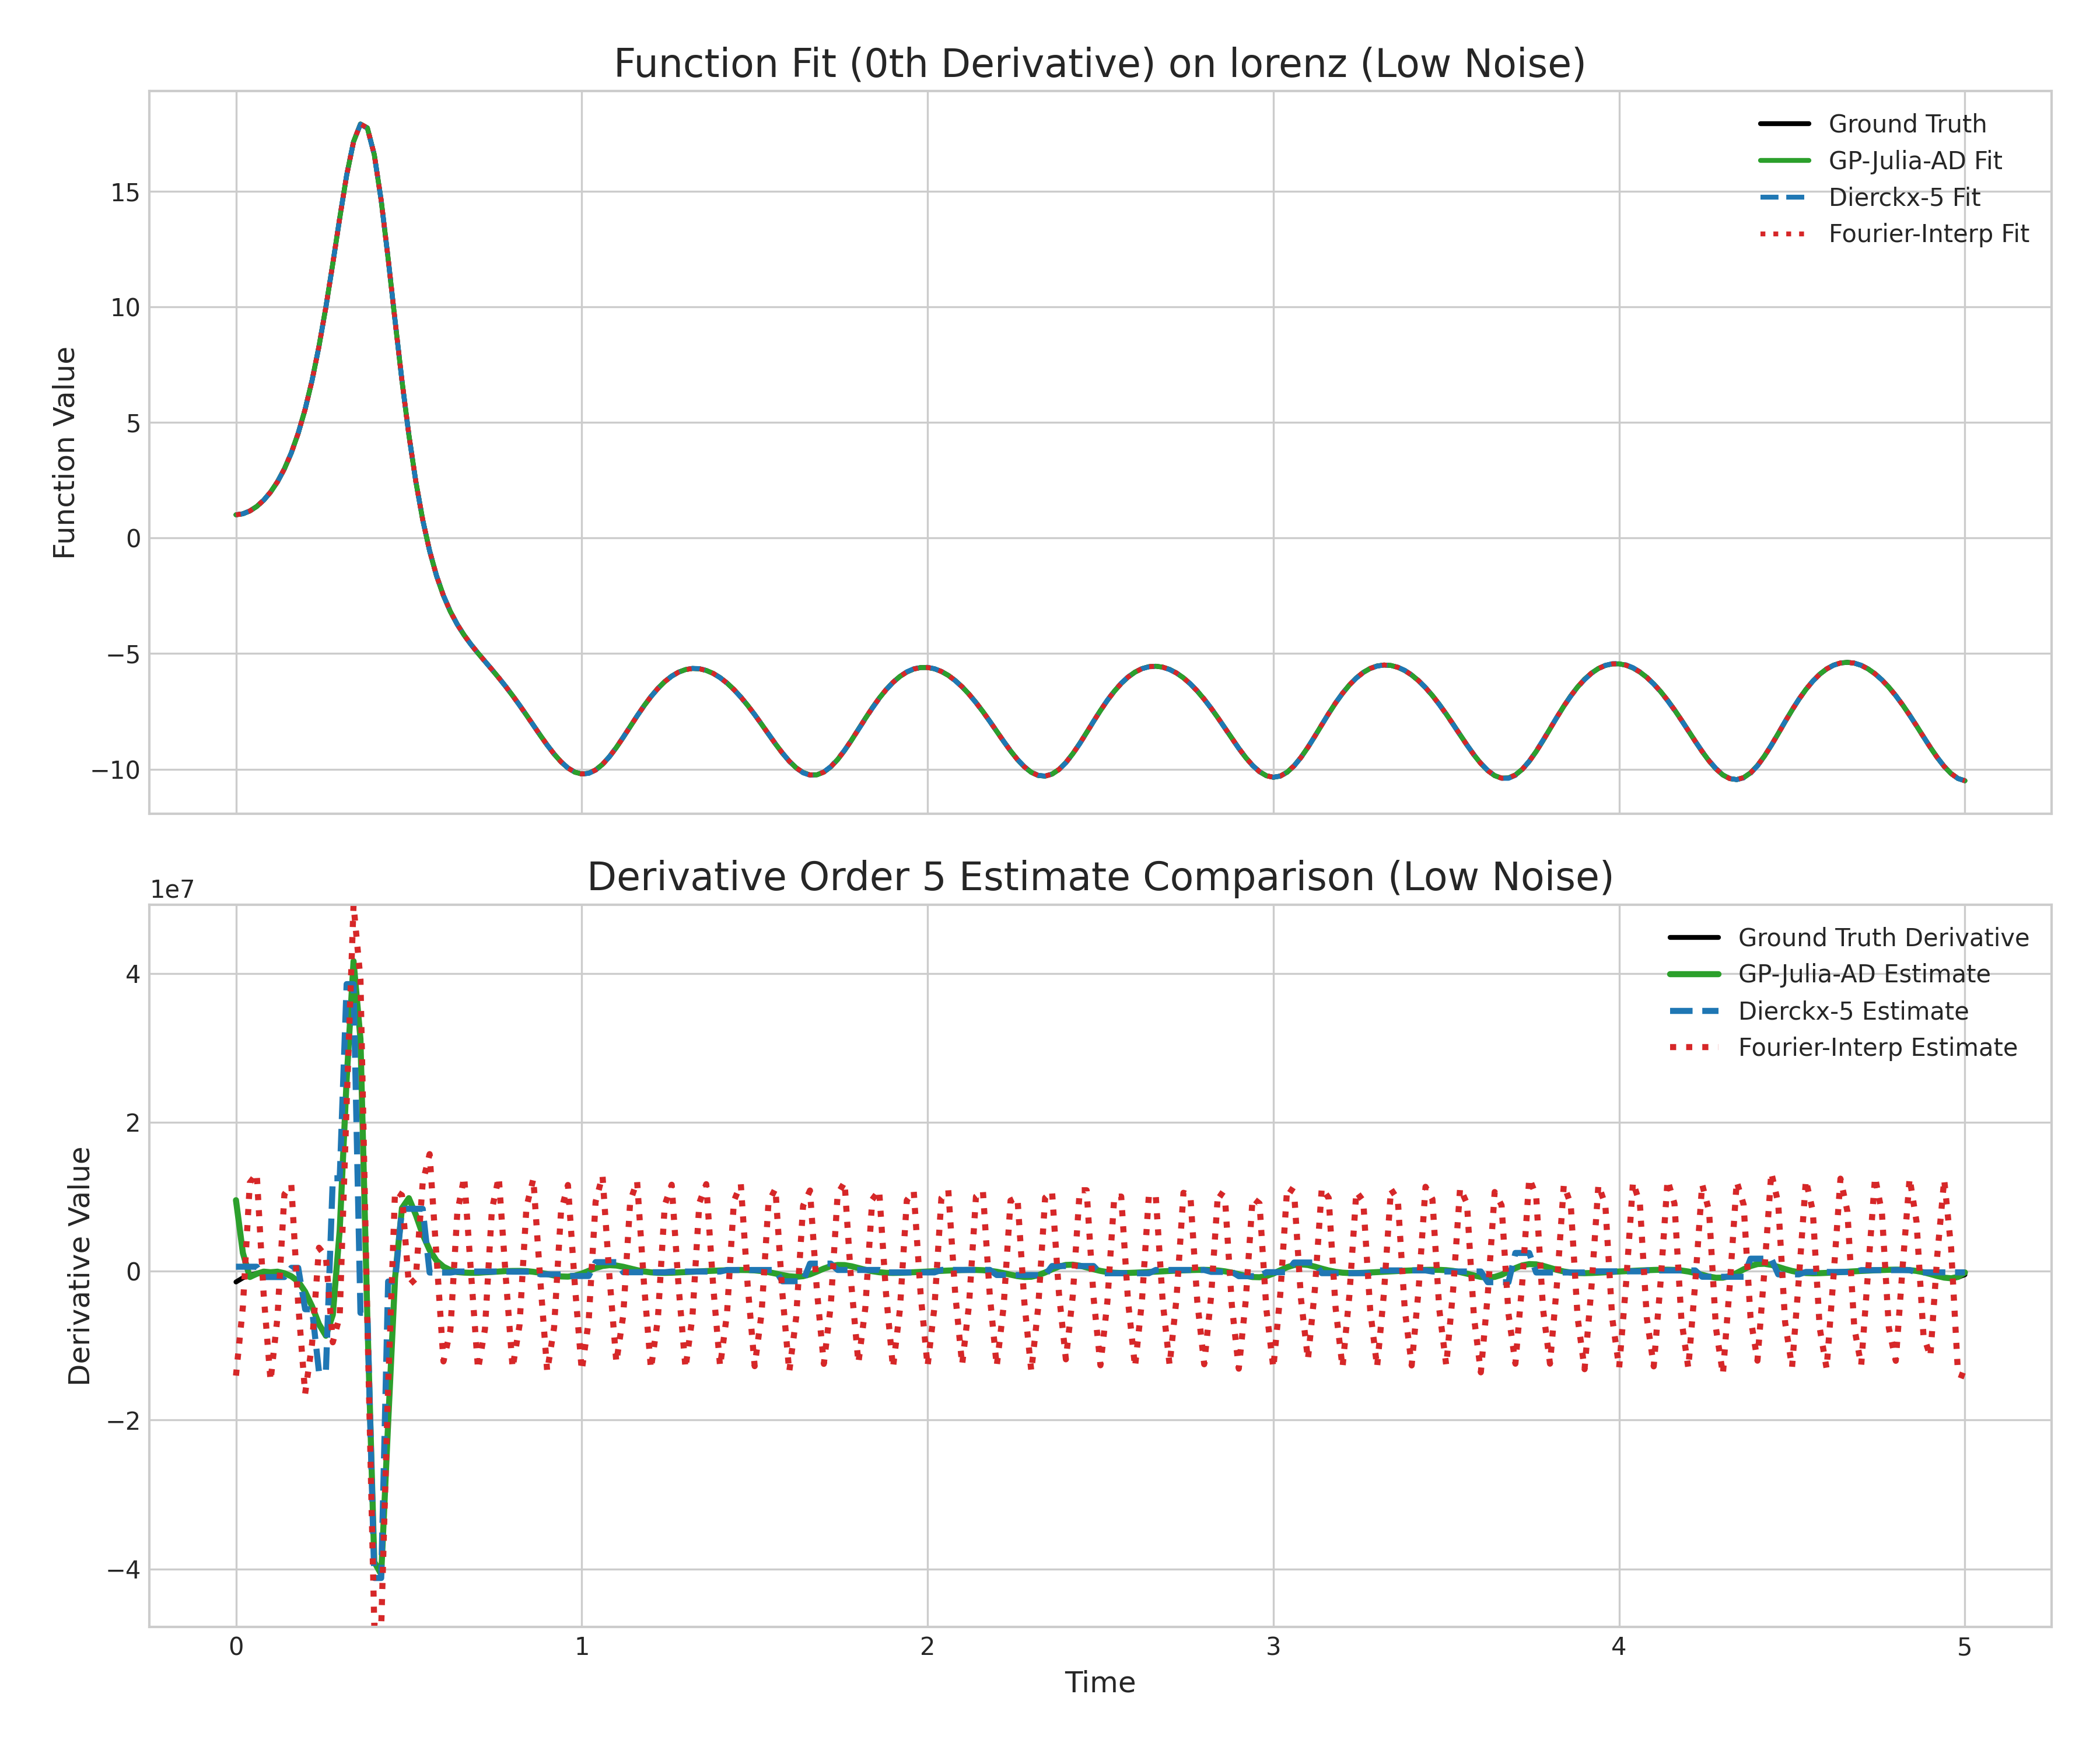
\includegraphics[width=0.9\textwidth]{low_noise_fit_comparison.png}
%\caption{\textbf{Low-Noise Precision.} In a low-noise environment (1e-8), this figure shows that for a 5th-order derivative, precision-focused methods become highly competitive. \texttt{Dierckx-5} (a smoothing spline) and \texttt{Fourier-Interp} (a spectral method) match the performance of \texttt{GP-Julia-AD}, illustrating that GPR's main advantage lies in its robustness to noise.}
%\label{fig:low_noise_comp}
%\end{figure}

\begin{figure}[htbp]
\centering
\includegraphics[width=0.9\textwidth]{top_methods_heatmap.png}
\caption{\textbf{Performance Degradation with Increasing Derivative Order.} This heatmap shows the mean nRMSE for top methods at a 1\% noise level. The vertical axis is sorted by average performance across all orders. This visualization clearly shows that \texttt{GP-Julia-AD} maintains low error across all derivative orders, while other methods like \texttt{Dierckx-5} and \texttt{GSS} are highly accurate for low orders but degrade significantly as the order increases.}
\label{fig:heatmap}
\end{figure}

\begin{figure}[htbp]
\centering
\includegraphics[width=0.9\textwidth]{pareto_frontier.png}
\caption{\textbf{Speed vs. Accuracy Trade-off.} For practitioners, the choice of method often involves a trade-off between computational cost and accuracy. This plot visualizes that trade-off for the contender methods. The black line represents the "Pareto Front"—the set of methods that are optimally efficient. Methods on this line represent the best possible accuracy for a given level of computational cost (or the fastest method for a given level of accuracy). This allows a practitioner to select a method that aligns with their specific computational budget and accuracy requirements. The plot clearly shows that the GPR methods, while the most accurate, are also the most computationally expensive.}
\label{fig:pareto}
\end{figure}
